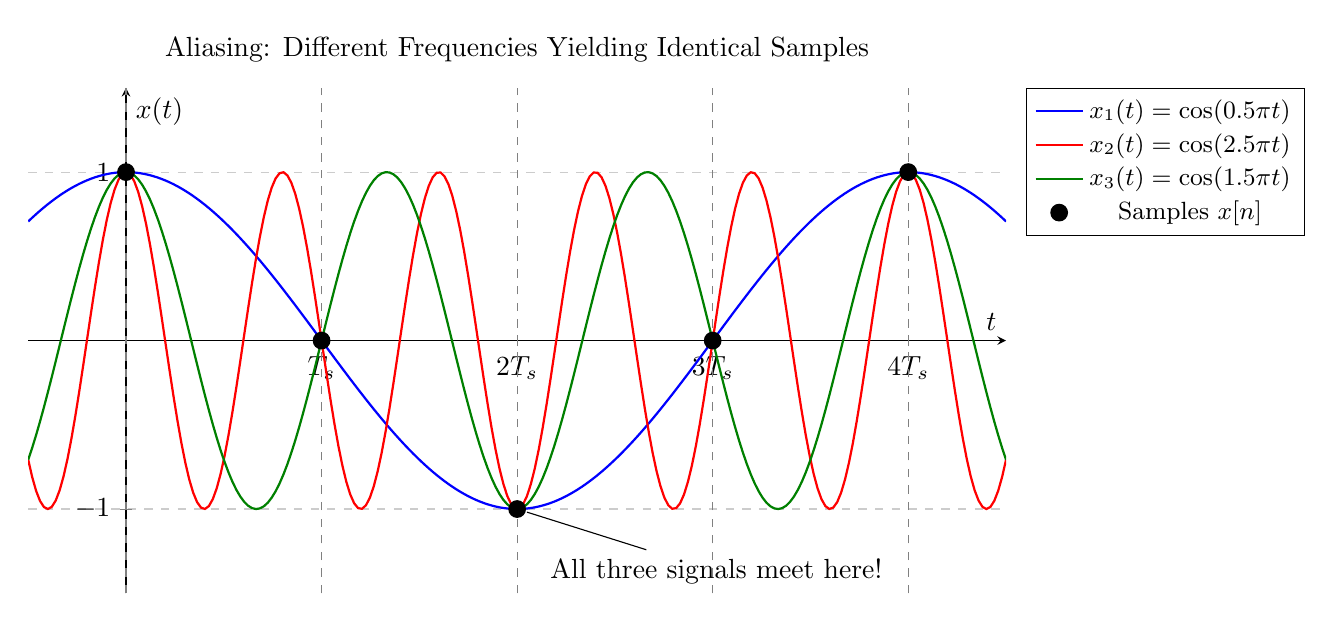
\begin{tikzpicture}
	\begin{axis}[
		width=14cm, 
		height=8cm,
		title={Aliasing: Different Frequencies Yielding Identical Samples},
		xlabel={$t$},
		ylabel={$x(t)$},
		axis lines=middle,
		xmin=-0.5, xmax=4.5,
		ymin=-1.5, ymax=1.5,
		xtick={0,1,2,3,4},
		xticklabels={$0$, $T_s$, $2T_s$, $3T_s$, $4T_s$},
		ytick={-1,1},
		grid=major,
		grid style={dashed, gray!40},
		legend style={at={(1.02,1)}, anchor=north west, font=\small},
		no marks,
		]
		% Signal 1 (Baseband Signal, f < f_N)
		\addplot[thick, blue, domain=-0.5:4.5, samples=250] {cos(deg(0.5*pi*x))};
		\addlegendentry{$x_1(t) = \cos(0.5\pi t)$};
		
		% Signal 2 (Alias, f > f_N)
		\addplot[thick, red, domain=-0.5:4.5, samples=250] {cos(deg(2.5*pi*x))};
		\addlegendentry{$x_2(t) = \cos(2.5\pi t)$};
		
		% Signal 3 (Another Alias, f > f_N)
		\addplot[thick, green!50!black, domain=-0.5:4.5, samples=250] {cos(deg(1.5*pi*x))};
		\addlegendentry{$x_3(t) = \cos(1.5\pi t)$};
		
		% Plot sample points
		\addplot[only marks, mark=*, mark size=3pt, black] coordinates {
			(0,1) (1,0) (2,-1) (3,0) (4,1)
		};
		\addlegendentry{Samples $x[n]$};
		
		% Vertical lines at sample positions
		\draw [gray, dashed] (axis cs:0,-1.5) -- (axis cs:0,1.5);
		\draw [gray, dashed] (axis cs:1,-1.5) -- (axis cs:1,1.5);
		\draw [gray, dashed] (axis cs:2,-1.5) -- (axis cs:2,1.5);
		\draw [gray, dashed] (axis cs:3,-1.5) -- (axis cs:3,1.5);
		\draw [gray, dashed] (axis cs:4,-1.5) -- (axis cs:4,1.5);
		
		% Add annotations
		\node[pin={[pin edge={black, thin}]-60:{All three signals meet here!}}] at (axis cs:2,-1) {};
		\node[above, font=\small, text width=5cm, align=center] at (axis description cs:0.5, 1.02) 
		{Sampling at $f_s = 1/T_s = 1$ Hz (Nyquist Freq. $f_N=0.5$ Hz)};
	\end{axis}
\end{tikzpicture}



